% Options for packages loaded elsewhere
% Options for packages loaded elsewhere
\PassOptionsToPackage{unicode}{hyperref}
\PassOptionsToPackage{hyphens}{url}
\PassOptionsToPackage{dvipsnames,svgnames,x11names}{xcolor}
%
\documentclass[
  english,
  letterpaper,
  DIV=11,
  numbers=noendperiod]{scrartcl}
\usepackage{xcolor}
\usepackage{amsmath,amssymb}
\setcounter{secnumdepth}{-\maxdimen} % remove section numbering
\usepackage{iftex}
\ifPDFTeX
  \usepackage[T1]{fontenc}
  \usepackage[utf8]{inputenc}
  \usepackage{textcomp} % provide euro and other symbols
\else % if luatex or xetex
  \usepackage{unicode-math} % this also loads fontspec
  \defaultfontfeatures{Scale=MatchLowercase}
  \defaultfontfeatures[\rmfamily]{Ligatures=TeX,Scale=1}
\fi
\usepackage{lmodern}
\ifPDFTeX\else
  % xetex/luatex font selection
\fi
% Use upquote if available, for straight quotes in verbatim environments
\IfFileExists{upquote.sty}{\usepackage{upquote}}{}
\IfFileExists{microtype.sty}{% use microtype if available
  \usepackage[]{microtype}
  \UseMicrotypeSet[protrusion]{basicmath} % disable protrusion for tt fonts
}{}
\makeatletter
\@ifundefined{KOMAClassName}{% if non-KOMA class
  \IfFileExists{parskip.sty}{%
    \usepackage{parskip}
  }{% else
    \setlength{\parindent}{0pt}
    \setlength{\parskip}{6pt plus 2pt minus 1pt}}
}{% if KOMA class
  \KOMAoptions{parskip=half}}
\makeatother
% Make \paragraph and \subparagraph free-standing
\makeatletter
\ifx\paragraph\undefined\else
  \let\oldparagraph\paragraph
  \renewcommand{\paragraph}{
    \@ifstar
      \xxxParagraphStar
      \xxxParagraphNoStar
  }
  \newcommand{\xxxParagraphStar}[1]{\oldparagraph*{#1}\mbox{}}
  \newcommand{\xxxParagraphNoStar}[1]{\oldparagraph{#1}\mbox{}}
\fi
\ifx\subparagraph\undefined\else
  \let\oldsubparagraph\subparagraph
  \renewcommand{\subparagraph}{
    \@ifstar
      \xxxSubParagraphStar
      \xxxSubParagraphNoStar
  }
  \newcommand{\xxxSubParagraphStar}[1]{\oldsubparagraph*{#1}\mbox{}}
  \newcommand{\xxxSubParagraphNoStar}[1]{\oldsubparagraph{#1}\mbox{}}
\fi
\makeatother

\usepackage{color}
\usepackage{fancyvrb}
\newcommand{\VerbBar}{|}
\newcommand{\VERB}{\Verb[commandchars=\\\{\}]}
\DefineVerbatimEnvironment{Highlighting}{Verbatim}{commandchars=\\\{\}}
% Add ',fontsize=\small' for more characters per line
\usepackage{framed}
\definecolor{shadecolor}{RGB}{241,243,245}
\newenvironment{Shaded}{\begin{snugshade}}{\end{snugshade}}
\newcommand{\AlertTok}[1]{\textcolor[rgb]{0.68,0.00,0.00}{#1}}
\newcommand{\AnnotationTok}[1]{\textcolor[rgb]{0.37,0.37,0.37}{#1}}
\newcommand{\AttributeTok}[1]{\textcolor[rgb]{0.40,0.45,0.13}{#1}}
\newcommand{\BaseNTok}[1]{\textcolor[rgb]{0.68,0.00,0.00}{#1}}
\newcommand{\BuiltInTok}[1]{\textcolor[rgb]{0.00,0.23,0.31}{#1}}
\newcommand{\CharTok}[1]{\textcolor[rgb]{0.13,0.47,0.30}{#1}}
\newcommand{\CommentTok}[1]{\textcolor[rgb]{0.37,0.37,0.37}{#1}}
\newcommand{\CommentVarTok}[1]{\textcolor[rgb]{0.37,0.37,0.37}{\textit{#1}}}
\newcommand{\ConstantTok}[1]{\textcolor[rgb]{0.56,0.35,0.01}{#1}}
\newcommand{\ControlFlowTok}[1]{\textcolor[rgb]{0.00,0.23,0.31}{\textbf{#1}}}
\newcommand{\DataTypeTok}[1]{\textcolor[rgb]{0.68,0.00,0.00}{#1}}
\newcommand{\DecValTok}[1]{\textcolor[rgb]{0.68,0.00,0.00}{#1}}
\newcommand{\DocumentationTok}[1]{\textcolor[rgb]{0.37,0.37,0.37}{\textit{#1}}}
\newcommand{\ErrorTok}[1]{\textcolor[rgb]{0.68,0.00,0.00}{#1}}
\newcommand{\ExtensionTok}[1]{\textcolor[rgb]{0.00,0.23,0.31}{#1}}
\newcommand{\FloatTok}[1]{\textcolor[rgb]{0.68,0.00,0.00}{#1}}
\newcommand{\FunctionTok}[1]{\textcolor[rgb]{0.28,0.35,0.67}{#1}}
\newcommand{\ImportTok}[1]{\textcolor[rgb]{0.00,0.46,0.62}{#1}}
\newcommand{\InformationTok}[1]{\textcolor[rgb]{0.37,0.37,0.37}{#1}}
\newcommand{\KeywordTok}[1]{\textcolor[rgb]{0.00,0.23,0.31}{\textbf{#1}}}
\newcommand{\NormalTok}[1]{\textcolor[rgb]{0.00,0.23,0.31}{#1}}
\newcommand{\OperatorTok}[1]{\textcolor[rgb]{0.37,0.37,0.37}{#1}}
\newcommand{\OtherTok}[1]{\textcolor[rgb]{0.00,0.23,0.31}{#1}}
\newcommand{\PreprocessorTok}[1]{\textcolor[rgb]{0.68,0.00,0.00}{#1}}
\newcommand{\RegionMarkerTok}[1]{\textcolor[rgb]{0.00,0.23,0.31}{#1}}
\newcommand{\SpecialCharTok}[1]{\textcolor[rgb]{0.37,0.37,0.37}{#1}}
\newcommand{\SpecialStringTok}[1]{\textcolor[rgb]{0.13,0.47,0.30}{#1}}
\newcommand{\StringTok}[1]{\textcolor[rgb]{0.13,0.47,0.30}{#1}}
\newcommand{\VariableTok}[1]{\textcolor[rgb]{0.07,0.07,0.07}{#1}}
\newcommand{\VerbatimStringTok}[1]{\textcolor[rgb]{0.13,0.47,0.30}{#1}}
\newcommand{\WarningTok}[1]{\textcolor[rgb]{0.37,0.37,0.37}{\textit{#1}}}

\usepackage{longtable,booktabs,array}
\usepackage{calc} % for calculating minipage widths
% Correct order of tables after \paragraph or \subparagraph
\usepackage{etoolbox}
\makeatletter
\patchcmd\longtable{\par}{\if@noskipsec\mbox{}\fi\par}{}{}
\makeatother
% Allow footnotes in longtable head/foot
\IfFileExists{footnotehyper.sty}{\usepackage{footnotehyper}}{\usepackage{footnote}}
\makesavenoteenv{longtable}
\usepackage{graphicx}
\makeatletter
\newsavebox\pandoc@box
\newcommand*\pandocbounded[1]{% scales image to fit in text height/width
  \sbox\pandoc@box{#1}%
  \Gscale@div\@tempa{\textheight}{\dimexpr\ht\pandoc@box+\dp\pandoc@box\relax}%
  \Gscale@div\@tempb{\linewidth}{\wd\pandoc@box}%
  \ifdim\@tempb\p@<\@tempa\p@\let\@tempa\@tempb\fi% select the smaller of both
  \ifdim\@tempa\p@<\p@\scalebox{\@tempa}{\usebox\pandoc@box}%
  \else\usebox{\pandoc@box}%
  \fi%
}
% Set default figure placement to htbp
\def\fps@figure{htbp}
\makeatother



\ifLuaTeX
\usepackage[bidi=basic]{babel}
\else
\usepackage[bidi=default]{babel}
\fi
% get rid of language-specific shorthands (see #6817):
\let\LanguageShortHands\languageshorthands
\def\languageshorthands#1{}
\ifLuaTeX
  \usepackage[english]{selnolig} % disable illegal ligatures
\fi


\setlength{\emergencystretch}{3em} % prevent overfull lines

\providecommand{\tightlist}{%
  \setlength{\itemsep}{0pt}\setlength{\parskip}{0pt}}



 


\KOMAoption{captions}{tableheading}
\makeatletter
\@ifpackageloaded{caption}{}{\usepackage{caption}}
\AtBeginDocument{%
\ifdefined\contentsname
  \renewcommand*\contentsname{Table of contents}
\else
  \newcommand\contentsname{Table of contents}
\fi
\ifdefined\listfigurename
  \renewcommand*\listfigurename{List of Figures}
\else
  \newcommand\listfigurename{List of Figures}
\fi
\ifdefined\listtablename
  \renewcommand*\listtablename{List of Tables}
\else
  \newcommand\listtablename{List of Tables}
\fi
\ifdefined\figurename
  \renewcommand*\figurename{Figure}
\else
  \newcommand\figurename{Figure}
\fi
\ifdefined\tablename
  \renewcommand*\tablename{Table}
\else
  \newcommand\tablename{Table}
\fi
}
\@ifpackageloaded{float}{}{\usepackage{float}}
\floatstyle{ruled}
\@ifundefined{c@chapter}{\newfloat{codelisting}{h}{lop}}{\newfloat{codelisting}{h}{lop}[chapter]}
\floatname{codelisting}{Listing}
\newcommand*\listoflistings{\listof{codelisting}{List of Listings}}
\makeatother
\makeatletter
\makeatother
\makeatletter
\@ifpackageloaded{caption}{}{\usepackage{caption}}
\@ifpackageloaded{subcaption}{}{\usepackage{subcaption}}
\makeatother
\usepackage{bookmark}
\IfFileExists{xurl.sty}{\usepackage{xurl}}{} % add URL line breaks if available
\urlstyle{same}
\hypersetup{
  pdftitle={Tarea N°4 Método de la Bisección},
  pdfauthor={Tamara Benavidez},
  pdflang={en},
  colorlinks=true,
  linkcolor={blue},
  filecolor={Maroon},
  citecolor={Blue},
  urlcolor={Blue},
  pdfcreator={LaTeX via pandoc}}


\title{Tarea N°4 Método de la Bisección}
\author{Tamara Benavidez}
\date{}
\begin{document}
\maketitle

\renewcommand*\contentsname{Tabla de Contenidos}
{
\hypersetup{linkcolor=}
\setcounter{tocdepth}{3}
\tableofcontents
}

\section{ESCUELA POLITÉCNICA
NACIONAL}\label{escuela-polituxe9cnica-nacional}

\begin{center}

\includegraphics[width=3cm,height=3cm]{logoEpn.jpg}
\end{center}

\section{TAREA N°4 Ejercicios Unidad 02
A}\label{tarea-n4-ejercicios-unidad-02-a}

\subsection{Método de la Bisección:
Ejercicios}\label{muxe9todo-de-la-bisecciuxf3n-ejercicios}

\begin{enumerate}
\def\labelenumi{\arabic{enumi}.}
\item
  Use el método de bisección para encontrar soluciones precisas dentro
  de \$ 10\^{}\{-2\}\$ para \$ x\^{}\{3\} -7x\^{}\{2\} + 14x-6=0\$ en
  cada intervalo.

  \begin{enumerate}
  \def\labelenumii{\alph{enumii}.}
  \item
    {[}0, 1{]}
  \item
    {[}1, 3.2{]}
  \item
    {[}3.2, 4{]}
  \end{enumerate}
\end{enumerate}

\begin{Shaded}
\begin{Highlighting}[]
\KeywordTok{def}\NormalTok{ biseccion(f, a, b, tol}\OperatorTok{=}\FloatTok{1e{-}2}\NormalTok{, max\_iter}\OperatorTok{=}\DecValTok{100}\NormalTok{):}
    
    \ControlFlowTok{if}\NormalTok{ f(a)}\OperatorTok{*}\NormalTok{f(b) }\OperatorTok{\textgreater{}} \DecValTok{0}\NormalTok{:}
        \ControlFlowTok{return} \VariableTok{None}\NormalTok{, }\DecValTok{0}  \CommentTok{\# No hay cambio de signo}
    
    \ControlFlowTok{for}\NormalTok{ i }\KeywordTok{in} \BuiltInTok{range}\NormalTok{(max\_iter):}
\NormalTok{        c }\OperatorTok{=}\NormalTok{ (a }\OperatorTok{+}\NormalTok{ b)}\OperatorTok{/}\DecValTok{2}
        \ControlFlowTok{if}\NormalTok{ f(c) }\OperatorTok{==} \DecValTok{0} \KeywordTok{or}\NormalTok{ (b }\OperatorTok{{-}}\NormalTok{ a)}\OperatorTok{/}\DecValTok{2} \OperatorTok{\textless{}}\NormalTok{ tol:}
            \ControlFlowTok{return}\NormalTok{ c, i}\OperatorTok{+}\DecValTok{1}
        \ControlFlowTok{if}\NormalTok{ f(a)}\OperatorTok{*}\NormalTok{f(c) }\OperatorTok{\textless{}} \DecValTok{0}\NormalTok{:}
\NormalTok{            b }\OperatorTok{=}\NormalTok{ c}
        \ControlFlowTok{else}\NormalTok{:}
\NormalTok{            a }\OperatorTok{=}\NormalTok{ c}
    \ControlFlowTok{return}\NormalTok{ (a}\OperatorTok{+}\NormalTok{b)}\OperatorTok{/}\DecValTok{2}\NormalTok{, max\_iter}

\CommentTok{\# Función}
\NormalTok{f }\OperatorTok{=} \KeywordTok{lambda}\NormalTok{ x: x}\OperatorTok{**}\DecValTok{3} \OperatorTok{{-}} \DecValTok{7}\OperatorTok{*}\NormalTok{x}\OperatorTok{**}\DecValTok{2} \OperatorTok{+} \DecValTok{14}\OperatorTok{*}\NormalTok{x }\OperatorTok{{-}} \DecValTok{6}

\CommentTok{\# Intervalos}
\NormalTok{intervalos }\OperatorTok{=}\NormalTok{ \{}
    \StringTok{"a"}\NormalTok{: (}\DecValTok{0}\NormalTok{, }\DecValTok{1}\NormalTok{),}
    \StringTok{"b"}\NormalTok{: (}\DecValTok{1}\NormalTok{, }\FloatTok{3.2}\NormalTok{),}
    \StringTok{"c"}\NormalTok{: (}\FloatTok{3.2}\NormalTok{, }\DecValTok{4}\NormalTok{)}
\NormalTok{\}}

\CommentTok{\# Se aplica el método de Bisección a cada intervalo}
\ControlFlowTok{for}\NormalTok{ key, (a, b) }\KeywordTok{in}\NormalTok{ intervalos.items():}
\NormalTok{    raiz, iteraciones }\OperatorTok{=}\NormalTok{ biseccion(f, a, b)}
    \BuiltInTok{print}\NormalTok{(}\SpecialStringTok{f"Raíz }\SpecialCharTok{\{}\NormalTok{key}\SpecialCharTok{\}}\SpecialStringTok{: }\SpecialCharTok{\{}\NormalTok{raiz}\SpecialCharTok{:.4f\}}\SpecialStringTok{ encontrada en }\SpecialCharTok{\{}\NormalTok{iteraciones}\SpecialCharTok{\}}\SpecialStringTok{ iteraciones"}\NormalTok{)}
\end{Highlighting}
\end{Shaded}

\begin{verbatim}
Raíz a: 0.5859 encontrada en 7 iteraciones
Raíz b: 3.0023 encontrada en 8 iteraciones
Raíz c: 3.4188 encontrada en 7 iteraciones
\end{verbatim}

\begin{enumerate}
\def\labelenumi{\arabic{enumi}.}
\setcounter{enumi}{1}
\tightlist
\item
  \begin{enumerate}
  \def\labelenumii{\alph{enumii}.}
  \tightlist
  \item
    Dibuje las gráficas para 𝑦 = 𝑥 y 𝑦 = sin x.
  \end{enumerate}
\end{enumerate}

\begin{Shaded}
\begin{Highlighting}[]
\ImportTok{import}\NormalTok{ numpy }\ImportTok{as}\NormalTok{ np}
\ImportTok{import}\NormalTok{ matplotlib.pyplot }\ImportTok{as}\NormalTok{ plt}

\NormalTok{x }\OperatorTok{=}\NormalTok{ np.linspace(}\DecValTok{0}\NormalTok{, }\DecValTok{2}\NormalTok{, }\DecValTok{400}\NormalTok{)}
\NormalTok{y1 }\OperatorTok{=}\NormalTok{ x}
\NormalTok{y2 }\OperatorTok{=}\NormalTok{ np.sin(x)}

\NormalTok{plt.figure(figsize}\OperatorTok{=}\NormalTok{(}\DecValTok{6}\NormalTok{,}\DecValTok{4}\NormalTok{))}
\NormalTok{plt.plot(x, y1, label}\OperatorTok{=}\StringTok{\textquotesingle{}y = x\textquotesingle{}}\NormalTok{)}
\NormalTok{plt.plot(x, y2, label}\OperatorTok{=}\StringTok{\textquotesingle{}y = sin(x)\textquotesingle{}}\NormalTok{)}
\NormalTok{plt.xlabel(}\StringTok{\textquotesingle{}x\textquotesingle{}}\NormalTok{)}
\NormalTok{plt.ylabel(}\StringTok{\textquotesingle{}y\textquotesingle{}}\NormalTok{)}
\NormalTok{plt.title(}\StringTok{\textquotesingle{}Gráfica de y = x y y = sin(x)\textquotesingle{}}\NormalTok{)}
\NormalTok{plt.grid(}\VariableTok{True}\NormalTok{)}
\NormalTok{plt.legend()}
\NormalTok{plt.show()}
\end{Highlighting}
\end{Shaded}

\pandocbounded{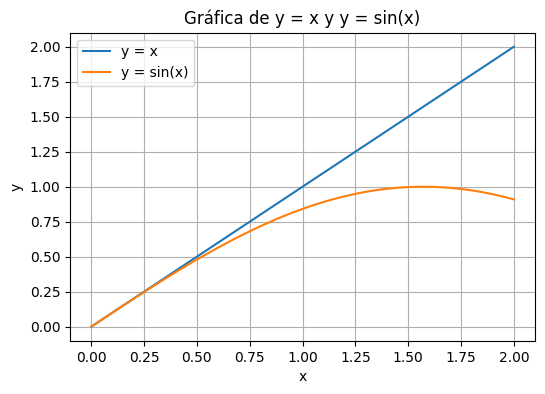
\includegraphics[keepaspectratio]{EjerciciosUnidad02A_files/figure-pdf/cell-3-output-1.png}}

\begin{verbatim}
b. Use el método de bisección para encontrar soluciones precisas dentro de $10^{-5} $ para el primer valor positivo de  x con $x = 2 sin x $.
\end{verbatim}

\begin{Shaded}
\begin{Highlighting}[]
\KeywordTok{def}\NormalTok{ biseccion(f, a, b, tol}\OperatorTok{=}\FloatTok{1e{-}5}\NormalTok{, max\_iter}\OperatorTok{=}\DecValTok{100}\NormalTok{):}
    \ControlFlowTok{if}\NormalTok{ f(a)}\OperatorTok{*}\NormalTok{f(b) }\OperatorTok{\textgreater{}} \DecValTok{0}\NormalTok{:}
        \ControlFlowTok{return} \VariableTok{None}\NormalTok{, }\DecValTok{0}  \CommentTok{\# No hay cambio de signo}
    \ControlFlowTok{for}\NormalTok{ i }\KeywordTok{in} \BuiltInTok{range}\NormalTok{(max\_iter):}
\NormalTok{        c }\OperatorTok{=}\NormalTok{ (a }\OperatorTok{+}\NormalTok{ b)}\OperatorTok{/}\DecValTok{2}
        \ControlFlowTok{if}\NormalTok{ f(c) }\OperatorTok{==} \DecValTok{0} \KeywordTok{or}\NormalTok{ (b }\OperatorTok{{-}}\NormalTok{ a)}\OperatorTok{/}\DecValTok{2} \OperatorTok{\textless{}}\NormalTok{ tol:}
            \ControlFlowTok{return}\NormalTok{ c, i}\OperatorTok{+}\DecValTok{1}
        \ControlFlowTok{if}\NormalTok{ f(a)}\OperatorTok{*}\NormalTok{f(c) }\OperatorTok{\textless{}} \DecValTok{0}\NormalTok{:}
\NormalTok{            b }\OperatorTok{=}\NormalTok{ c}
        \ControlFlowTok{else}\NormalTok{:}
\NormalTok{            a }\OperatorTok{=}\NormalTok{ c}
    \ControlFlowTok{return}\NormalTok{ (a}\OperatorTok{+}\NormalTok{b)}\OperatorTok{/}\DecValTok{2}\NormalTok{, max\_iter}

\CommentTok{\# Función f(x) = x {-} 2*sin(x)}
\NormalTok{f }\OperatorTok{=} \KeywordTok{lambda}\NormalTok{ x: x }\OperatorTok{{-}} \DecValTok{2}\OperatorTok{*}\NormalTok{np.sin(x)}

\CommentTok{\# Primer cero positivo}
\NormalTok{raiz, iteraciones }\OperatorTok{=}\NormalTok{ biseccion(f, }\DecValTok{0}\NormalTok{, }\DecValTok{2}\NormalTok{)}
\BuiltInTok{print}\NormalTok{(}\SpecialStringTok{f"Primer cero positivo: x = }\SpecialCharTok{\{}\NormalTok{raiz}\SpecialCharTok{:.5f\}}\SpecialStringTok{ encontrado en }\SpecialCharTok{\{}\NormalTok{iteraciones}\SpecialCharTok{\}}\SpecialStringTok{ iteraciones"}\NormalTok{)}
\end{Highlighting}
\end{Shaded}

\begin{verbatim}
Primer cero positivo: x = 1.89550 encontrado en 18 iteraciones
\end{verbatim}

\begin{enumerate}
\def\labelenumi{\arabic{enumi}.}
\setcounter{enumi}{2}
\tightlist
\item
  \begin{enumerate}
  \def\labelenumii{\alph{enumii}.}
  \tightlist
  \item
    Dibuje las gráficas para \$ y = x \$ y \$ y = tan x \$
  \end{enumerate}
\end{enumerate}

\begin{Shaded}
\begin{Highlighting}[]
\ImportTok{import}\NormalTok{ numpy }\ImportTok{as}\NormalTok{ np}
\ImportTok{import}\NormalTok{ matplotlib.pyplot }\ImportTok{as}\NormalTok{ plt}

\NormalTok{x }\OperatorTok{=}\NormalTok{ np.linspace(}\DecValTok{0}\NormalTok{, }\FloatTok{1.4}\NormalTok{, }\DecValTok{400}\NormalTok{)  }\CommentTok{\# evitamos pi/2 porque tan(x) → ∞}
\NormalTok{y1 }\OperatorTok{=}\NormalTok{ x}
\NormalTok{y2 }\OperatorTok{=}\NormalTok{ np.tan(x)}

\NormalTok{plt.figure(figsize}\OperatorTok{=}\NormalTok{(}\DecValTok{6}\NormalTok{,}\DecValTok{4}\NormalTok{))}
\NormalTok{plt.plot(x, y1, label}\OperatorTok{=}\StringTok{\textquotesingle{}y = x\textquotesingle{}}\NormalTok{)}
\NormalTok{plt.plot(x, y2, label}\OperatorTok{=}\StringTok{\textquotesingle{}y = tan(x)\textquotesingle{}}\NormalTok{)}
\NormalTok{plt.xlabel(}\StringTok{\textquotesingle{}x\textquotesingle{}}\NormalTok{)}
\NormalTok{plt.ylabel(}\StringTok{\textquotesingle{}y\textquotesingle{}}\NormalTok{)}
\NormalTok{plt.title(}\StringTok{\textquotesingle{}Gráfica de y = x y y = tan(x)\textquotesingle{}}\NormalTok{)}
\NormalTok{plt.grid(}\VariableTok{True}\NormalTok{)}
\NormalTok{plt.legend()}
\NormalTok{plt.ylim(}\OperatorTok{{-}}\DecValTok{5}\NormalTok{, }\DecValTok{5}\NormalTok{)  }\CommentTok{\# para que la curva de tan(x) se vea mejor}
\NormalTok{plt.show()}
\end{Highlighting}
\end{Shaded}

\pandocbounded{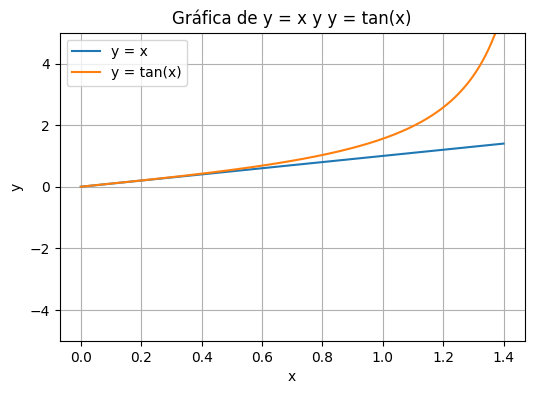
\includegraphics[keepaspectratio]{EjerciciosUnidad02A_files/figure-pdf/cell-5-output-1.png}}

\begin{verbatim}
b. Use el método de bisección para encontrar una aproximación dentro de $10^{-5}$  para el primer valor positivo  x con $x = tan x $
\end{verbatim}

\begin{Shaded}
\begin{Highlighting}[]
\KeywordTok{def}\NormalTok{ biseccion(f, a, b, tol}\OperatorTok{=}\FloatTok{1e{-}5}\NormalTok{, max\_iter}\OperatorTok{=}\DecValTok{100}\NormalTok{):}
    \ControlFlowTok{if}\NormalTok{ f(a)}\OperatorTok{*}\NormalTok{f(b) }\OperatorTok{\textgreater{}} \DecValTok{0}\NormalTok{:}
        \ControlFlowTok{return} \VariableTok{None}\NormalTok{, }\DecValTok{0}  \CommentTok{\# No hay cambio de signo}
    \ControlFlowTok{for}\NormalTok{ i }\KeywordTok{in} \BuiltInTok{range}\NormalTok{(max\_iter):}
\NormalTok{        c }\OperatorTok{=}\NormalTok{ (a }\OperatorTok{+}\NormalTok{ b)}\OperatorTok{/}\DecValTok{2}
        \ControlFlowTok{if}\NormalTok{ f(c) }\OperatorTok{==} \DecValTok{0} \KeywordTok{or}\NormalTok{ (b }\OperatorTok{{-}}\NormalTok{ a)}\OperatorTok{/}\DecValTok{2} \OperatorTok{\textless{}}\NormalTok{ tol:}
            \ControlFlowTok{return}\NormalTok{ c, i}\OperatorTok{+}\DecValTok{1}
        \ControlFlowTok{if}\NormalTok{ f(a)}\OperatorTok{*}\NormalTok{f(c) }\OperatorTok{\textless{}} \DecValTok{0}\NormalTok{:}
\NormalTok{            b }\OperatorTok{=}\NormalTok{ c}
        \ControlFlowTok{else}\NormalTok{:}
\NormalTok{            a }\OperatorTok{=}\NormalTok{ c}
    \ControlFlowTok{return}\NormalTok{ (a}\OperatorTok{+}\NormalTok{b)}\OperatorTok{/}\DecValTok{2}\NormalTok{, max\_iter}

\CommentTok{\# Función f(x) = x {-} tan(x)}
\NormalTok{f }\OperatorTok{=} \KeywordTok{lambda}\NormalTok{ x: x }\OperatorTok{{-}}\NormalTok{ np.tan(x)}

\CommentTok{\# Primer cero positivo (buscado antes de pi/2)}
\NormalTok{raiz, iteraciones }\OperatorTok{=}\NormalTok{ biseccion(f, }\DecValTok{0}\NormalTok{, }\FloatTok{1.4}\NormalTok{)}
\BuiltInTok{print}\NormalTok{(}\SpecialStringTok{f"Primer cero positivo: x = }\SpecialCharTok{\{}\NormalTok{raiz}\SpecialCharTok{:.5f\}}\SpecialStringTok{ encontrado en }\SpecialCharTok{\{}\NormalTok{iteraciones}\SpecialCharTok{\}}\SpecialStringTok{ iteraciones"}\NormalTok{)}
\end{Highlighting}
\end{Shaded}

\begin{verbatim}
Primer cero positivo: x = 1.39999 encontrado en 18 iteraciones
\end{verbatim}

\begin{enumerate}
\def\labelenumi{\arabic{enumi}.}
\setcounter{enumi}{3}
\tightlist
\item
  \begin{enumerate}
  \def\labelenumii{\alph{enumii}.}
  \tightlist
  \item
    Dibuje las gráficas para \$ y = x\^{}\{2\} -1\$ y \$ y =
    e\textsuperscript{\{1-x}\{2\}\}\$
  \end{enumerate}
\end{enumerate}

\begin{Shaded}
\begin{Highlighting}[]
\ImportTok{import}\NormalTok{ numpy }\ImportTok{as}\NormalTok{ np}
\ImportTok{import}\NormalTok{ matplotlib.pyplot }\ImportTok{as}\NormalTok{ plt}

\NormalTok{x }\OperatorTok{=}\NormalTok{ np.linspace(}\OperatorTok{{-}}\DecValTok{2}\NormalTok{, }\DecValTok{1}\NormalTok{, }\DecValTok{400}\NormalTok{)}
\NormalTok{y1 }\OperatorTok{=}\NormalTok{ x}\OperatorTok{**}\DecValTok{2} \OperatorTok{{-}} \DecValTok{1}
\NormalTok{y2 }\OperatorTok{=}\NormalTok{ np.exp(}\DecValTok{1} \OperatorTok{{-}}\NormalTok{ x}\OperatorTok{**}\DecValTok{2}\NormalTok{)}

\NormalTok{plt.figure(figsize}\OperatorTok{=}\NormalTok{(}\DecValTok{6}\NormalTok{,}\DecValTok{4}\NormalTok{))}
\NormalTok{plt.plot(x, y1, label}\OperatorTok{=}\StringTok{\textquotesingle{}y = x\^{}2 {-} 1\textquotesingle{}}\NormalTok{)}
\NormalTok{plt.plot(x, y2, label}\OperatorTok{=}\StringTok{\textquotesingle{}y = e\^{}(1 {-} x\^{}2)\textquotesingle{}}\NormalTok{)}
\NormalTok{plt.xlabel(}\StringTok{\textquotesingle{}x\textquotesingle{}}\NormalTok{)}
\NormalTok{plt.ylabel(}\StringTok{\textquotesingle{}y\textquotesingle{}}\NormalTok{)}
\NormalTok{plt.title(}\StringTok{\textquotesingle{}Gráfica de y = x\^{}2 {-} 1 y y = e\^{}(1 {-} x\^{}2)\textquotesingle{}}\NormalTok{)}
\NormalTok{plt.grid(}\VariableTok{True}\NormalTok{)}
\NormalTok{plt.legend()}
\NormalTok{plt.show()}
\end{Highlighting}
\end{Shaded}

\pandocbounded{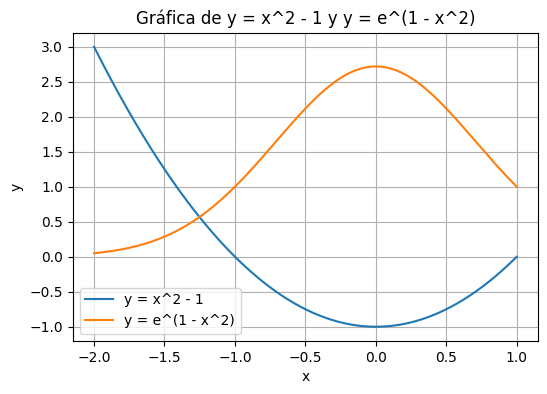
\includegraphics[keepaspectratio]{EjerciciosUnidad02A_files/figure-pdf/cell-7-output-1.png}}

\begin{verbatim}
b. Use el método de bisección para encontrar una aproximación dentro de $10 ^{-3} $  para un valor en [−2, 0] con $ x ^{2} -1 = e^{1-x^{2}} $.
\end{verbatim}

\begin{Shaded}
\begin{Highlighting}[]
\KeywordTok{def}\NormalTok{ biseccion(f, a, b, tol}\OperatorTok{=}\FloatTok{1e{-}3}\NormalTok{, max\_iter}\OperatorTok{=}\DecValTok{100}\NormalTok{):}
    \ControlFlowTok{if}\NormalTok{ f(a)}\OperatorTok{*}\NormalTok{f(b) }\OperatorTok{\textgreater{}} \DecValTok{0}\NormalTok{:}
        \ControlFlowTok{return} \VariableTok{None}\NormalTok{, }\DecValTok{0}  \CommentTok{\# No hay cambio de signo}
    \ControlFlowTok{for}\NormalTok{ i }\KeywordTok{in} \BuiltInTok{range}\NormalTok{(max\_iter):}
\NormalTok{        c }\OperatorTok{=}\NormalTok{ (a }\OperatorTok{+}\NormalTok{ b)}\OperatorTok{/}\DecValTok{2}
        \ControlFlowTok{if}\NormalTok{ f(c) }\OperatorTok{==} \DecValTok{0} \KeywordTok{or}\NormalTok{ (b }\OperatorTok{{-}}\NormalTok{ a)}\OperatorTok{/}\DecValTok{2} \OperatorTok{\textless{}}\NormalTok{ tol:}
            \ControlFlowTok{return}\NormalTok{ c, i}\OperatorTok{+}\DecValTok{1}
        \ControlFlowTok{if}\NormalTok{ f(a)}\OperatorTok{*}\NormalTok{f(c) }\OperatorTok{\textless{}} \DecValTok{0}\NormalTok{:}
\NormalTok{            b }\OperatorTok{=}\NormalTok{ c}
        \ControlFlowTok{else}\NormalTok{:}
\NormalTok{            a }\OperatorTok{=}\NormalTok{ c}
    \ControlFlowTok{return}\NormalTok{ (a}\OperatorTok{+}\NormalTok{b)}\OperatorTok{/}\DecValTok{2}\NormalTok{, max\_iter}

\CommentTok{\# Función f(x) = x\^{}2 {-} 1 {-} exp(1 {-} x\^{}2)}
\NormalTok{f }\OperatorTok{=} \KeywordTok{lambda}\NormalTok{ x: x}\OperatorTok{**}\DecValTok{2} \OperatorTok{{-}} \DecValTok{1} \OperatorTok{{-}}\NormalTok{ np.exp(}\DecValTok{1} \OperatorTok{{-}}\NormalTok{ x}\OperatorTok{**}\DecValTok{2}\NormalTok{)}

\CommentTok{\# Raíz en [{-}2, 0]}
\NormalTok{raiz, iteraciones }\OperatorTok{=}\NormalTok{ biseccion(f, }\OperatorTok{{-}}\DecValTok{2}\NormalTok{, }\DecValTok{0}\NormalTok{)}
\BuiltInTok{print}\NormalTok{(}\SpecialStringTok{f"Raíz en [{-}2,0]: x = }\SpecialCharTok{\{}\NormalTok{raiz}\SpecialCharTok{:.3f\}}\SpecialStringTok{ encontrada en }\SpecialCharTok{\{}\NormalTok{iteraciones}\SpecialCharTok{\}}\SpecialStringTok{ iteraciones"}\NormalTok{)}
\end{Highlighting}
\end{Shaded}

\begin{verbatim}
Raíz en [-2,0]: x = -1.251 encontrada en 11 iteraciones
\end{verbatim}

\begin{enumerate}
\def\labelenumi{\arabic{enumi}.}
\setcounter{enumi}{4}
\item
  Sea 𝑓(𝑥) = \((𝑥 + 3)(𝑥 + 1)^2 x (x-1)^3 (x-3)\) ¿En qué cero de 𝑓
  converge el método de bisección cuando se aplica en los siguientes
  intervalos?

  \begin{enumerate}
  \def\labelenumii{\alph{enumii}.}
  \item
    {[}-1.5, 2.5{]}
  \item
    {[}-0.5, 2.4{]}
  \item
    {[}-0.5, 3{]}
  \end{enumerate}
\end{enumerate}

\begin{Shaded}
\begin{Highlighting}[]
\KeywordTok{def}\NormalTok{ biseccion(f, a, b, tol}\OperatorTok{=}\FloatTok{1e{-}5}\NormalTok{, max\_iter}\OperatorTok{=}\DecValTok{100}\NormalTok{):}
    \ControlFlowTok{if}\NormalTok{ f(a)}\OperatorTok{*}\NormalTok{f(b) }\OperatorTok{\textgreater{}} \DecValTok{0}\NormalTok{:}
        \ControlFlowTok{return} \VariableTok{None}\NormalTok{, }\DecValTok{0}  \CommentTok{\# No hay cambio de signo}
    \ControlFlowTok{for}\NormalTok{ i }\KeywordTok{in} \BuiltInTok{range}\NormalTok{(max\_iter):}
\NormalTok{        c }\OperatorTok{=}\NormalTok{ (a }\OperatorTok{+}\NormalTok{ b)}\OperatorTok{/}\DecValTok{2}
        \ControlFlowTok{if}\NormalTok{ f(c) }\OperatorTok{==} \DecValTok{0} \KeywordTok{or}\NormalTok{ (b }\OperatorTok{{-}}\NormalTok{ a)}\OperatorTok{/}\DecValTok{2} \OperatorTok{\textless{}}\NormalTok{ tol:}
            \ControlFlowTok{return}\NormalTok{ c, i}\OperatorTok{+}\DecValTok{1}
        \ControlFlowTok{if}\NormalTok{ f(a)}\OperatorTok{*}\NormalTok{f(c) }\OperatorTok{\textless{}} \DecValTok{0}\NormalTok{:}
\NormalTok{            b }\OperatorTok{=}\NormalTok{ c}
        \ControlFlowTok{else}\NormalTok{:}
\NormalTok{            a }\OperatorTok{=}\NormalTok{ c}
    \ControlFlowTok{return}\NormalTok{ (a}\OperatorTok{+}\NormalTok{b)}\OperatorTok{/}\DecValTok{2}\NormalTok{, max\_iter}

\CommentTok{\# Función}
\NormalTok{f }\OperatorTok{=} \KeywordTok{lambda}\NormalTok{ x: (x }\OperatorTok{+} \DecValTok{3}\NormalTok{)}\OperatorTok{*}\NormalTok{(x }\OperatorTok{+} \DecValTok{1}\NormalTok{)}\OperatorTok{**}\DecValTok{2} \OperatorTok{*}\NormalTok{ x }\OperatorTok{*}\NormalTok{ (x }\OperatorTok{{-}} \DecValTok{1}\NormalTok{)}\OperatorTok{**}\DecValTok{3} \OperatorTok{*}\NormalTok{ (x }\OperatorTok{{-}} \DecValTok{3}\NormalTok{)}

\CommentTok{\# Intervalos}
\NormalTok{intervalos }\OperatorTok{=}\NormalTok{ \{}
    \StringTok{"a"}\NormalTok{: (}\OperatorTok{{-}}\FloatTok{1.5}\NormalTok{, }\FloatTok{2.5}\NormalTok{),}
    \StringTok{"b"}\NormalTok{: (}\OperatorTok{{-}}\FloatTok{0.5}\NormalTok{, }\FloatTok{2.4}\NormalTok{),}
    \StringTok{"c"}\NormalTok{: (}\OperatorTok{{-}}\FloatTok{0.5}\NormalTok{, }\DecValTok{3}\NormalTok{),}
    \StringTok{"d"}\NormalTok{: (}\OperatorTok{{-}}\DecValTok{3}\NormalTok{, }\OperatorTok{{-}}\FloatTok{0.5}\NormalTok{)}
\NormalTok{\}}

\CommentTok{\# Se aplica el método de Bisección a cada intervalo}
\ControlFlowTok{for}\NormalTok{ key, (a, b) }\KeywordTok{in}\NormalTok{ intervalos.items():}
\NormalTok{    raiz, iteraciones }\OperatorTok{=}\NormalTok{ biseccion(f, a, b)}
    \ControlFlowTok{if}\NormalTok{ raiz }\KeywordTok{is} \KeywordTok{not} \VariableTok{None}\NormalTok{:}
        \BuiltInTok{print}\NormalTok{(}\SpecialStringTok{f"Intervalo }\SpecialCharTok{\{}\NormalTok{key}\SpecialCharTok{\}}\SpecialStringTok{ [}\SpecialCharTok{\{}\NormalTok{a}\SpecialCharTok{\}}\SpecialStringTok{,}\SpecialCharTok{\{}\NormalTok{b}\SpecialCharTok{\}}\SpecialStringTok{] → raíz aproximada: }\SpecialCharTok{\{}\NormalTok{raiz}\SpecialCharTok{:.5f\}}\SpecialStringTok{ en }\SpecialCharTok{\{}\NormalTok{iteraciones}\SpecialCharTok{\}}\SpecialStringTok{ iteraciones"}\NormalTok{)}
    \ControlFlowTok{else}\NormalTok{:}
        \BuiltInTok{print}\NormalTok{(}\SpecialStringTok{f"Intervalo }\SpecialCharTok{\{}\NormalTok{key}\SpecialCharTok{\}}\SpecialStringTok{ [}\SpecialCharTok{\{}\NormalTok{a}\SpecialCharTok{\}}\SpecialStringTok{,}\SpecialCharTok{\{}\NormalTok{b}\SpecialCharTok{\}}\SpecialStringTok{] → No hay cambio de signo, no se encuentra raíz por bisección"}\NormalTok{)}
\end{Highlighting}
\end{Shaded}

\begin{verbatim}
Intervalo a [-1.5,2.5] → No hay cambio de signo, no se encuentra raíz por bisección
Intervalo b [-0.5,2.4] → No hay cambio de signo, no se encuentra raíz por bisección
Intervalo c [-0.5,3] → raíz aproximada: 2.99999 en 19 iteraciones
Intervalo d [-3,-0.5] → raíz aproximada: -0.50001 en 18 iteraciones
\end{verbatim}

\subsection{EJERCICIOS APLICADOS}\label{ejercicios-aplicados}

\begin{enumerate}
\def\labelenumi{\arabic{enumi}.}
\tightlist
\item
  Un abrevadero de longitud 𝐿 tiene una sección transversal en forma de
  semicírculo con radio 𝑟. (Consulte la figura adjunta.) Cuando se llena
  con agua hasta una distancia ℎ a partir de la parte superior, el
  volumen 𝑉 de agua es
\end{enumerate}

\$ V = L{[}0.5\pi r\^{}\{2\} - r\^{}\{2\}arcsen(h/r) -h(r\^{}2 -
h\textsuperscript{2)}\{\frac{1}{2}\}{]} \$

\begin{center}
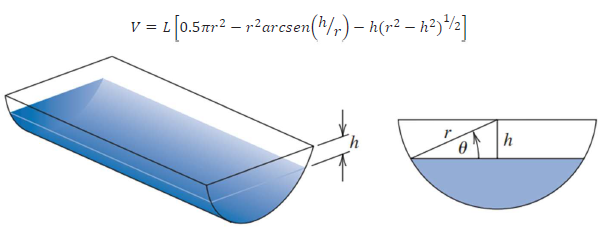
\includegraphics[width=7cm,height=5cm]{EjercicioA1.png}
\end{center}

Suponga que 𝐿 = 10 𝑐𝑚, 𝑟 = 1 𝑐𝑚 y 𝑉 = 12.4 \$cm\^{}\{3\} \$. Encuentre
la profundidad del agua en el abrevadero dentro de 0.01 𝑐𝑚.

\begin{Shaded}
\begin{Highlighting}[]
\ImportTok{import}\NormalTok{ numpy }\ImportTok{as}\NormalTok{ np}

\CommentTok{\# Datos}
\NormalTok{L }\OperatorTok{=} \DecValTok{10}  \CommentTok{\# cm}
\NormalTok{r }\OperatorTok{=} \DecValTok{1}   \CommentTok{\# cm}
\NormalTok{V\_obj }\OperatorTok{=} \FloatTok{12.4}  \CommentTok{\# cm\^{}3}

\CommentTok{\# Función f(h) = V(h) {-} V\_obj}
\KeywordTok{def}\NormalTok{ f(h):}
    \ControlFlowTok{return}\NormalTok{ L}\OperatorTok{*}\NormalTok{(}\FloatTok{0.5}\OperatorTok{*}\NormalTok{np.pi}\OperatorTok{*}\NormalTok{r}\OperatorTok{**}\DecValTok{2} \OperatorTok{{-}}\NormalTok{ r}\OperatorTok{**}\DecValTok{2}\OperatorTok{*}\NormalTok{np.arcsin(h}\OperatorTok{/}\NormalTok{r) }\OperatorTok{{-}}\NormalTok{ h}\OperatorTok{*}\NormalTok{np.sqrt(r}\OperatorTok{**}\DecValTok{2} \OperatorTok{{-}}\NormalTok{ h}\OperatorTok{**}\DecValTok{2}\NormalTok{)) }\OperatorTok{{-}}\NormalTok{ V\_obj}

\CommentTok{\# Método de Bisección}
\KeywordTok{def}\NormalTok{ biseccion(f, a, b, tol}\OperatorTok{=}\FloatTok{0.01}\NormalTok{, max\_iter}\OperatorTok{=}\DecValTok{100}\NormalTok{):}
    \ControlFlowTok{if}\NormalTok{ f(a)}\OperatorTok{*}\NormalTok{f(b) }\OperatorTok{\textgreater{}} \DecValTok{0}\NormalTok{:}
        \ControlFlowTok{return} \VariableTok{None}\NormalTok{, }\DecValTok{0}  \CommentTok{\# No hay cambio de signo}
    \ControlFlowTok{for}\NormalTok{ i }\KeywordTok{in} \BuiltInTok{range}\NormalTok{(max\_iter):}
\NormalTok{        c }\OperatorTok{=}\NormalTok{ (a }\OperatorTok{+}\NormalTok{ b)}\OperatorTok{/}\DecValTok{2}
        \ControlFlowTok{if}\NormalTok{ f(c) }\OperatorTok{==} \DecValTok{0} \KeywordTok{or}\NormalTok{ (b }\OperatorTok{{-}}\NormalTok{ a)}\OperatorTok{/}\DecValTok{2} \OperatorTok{\textless{}}\NormalTok{ tol:}
            \ControlFlowTok{return}\NormalTok{ c, i}\OperatorTok{+}\DecValTok{1}
        \ControlFlowTok{if}\NormalTok{ f(a)}\OperatorTok{*}\NormalTok{f(c) }\OperatorTok{\textless{}} \DecValTok{0}\NormalTok{:}
\NormalTok{            b }\OperatorTok{=}\NormalTok{ c}
        \ControlFlowTok{else}\NormalTok{:}
\NormalTok{            a }\OperatorTok{=}\NormalTok{ c}
    \ControlFlowTok{return}\NormalTok{ (a}\OperatorTok{+}\NormalTok{b)}\OperatorTok{/}\DecValTok{2}\NormalTok{, max\_iter}

\CommentTok{\# Intervalo posible [0, r]}
\NormalTok{raiz, iteraciones }\OperatorTok{=}\NormalTok{ biseccion(f, }\DecValTok{0}\NormalTok{, r)}
\BuiltInTok{print}\NormalTok{(}\SpecialStringTok{f"Profundidad del agua: h = }\SpecialCharTok{\{}\NormalTok{raiz}\SpecialCharTok{:.2f\}}\SpecialStringTok{ cm encontrada en }\SpecialCharTok{\{}\NormalTok{iteraciones}\SpecialCharTok{\}}\SpecialStringTok{ iteraciones"}\NormalTok{)}
\end{Highlighting}
\end{Shaded}

\begin{verbatim}
Profundidad del agua: h = 0.16 cm encontrada en 7 iteraciones
\end{verbatim}

\begin{enumerate}
\def\labelenumi{\arabic{enumi}.}
\setcounter{enumi}{1}
\tightlist
\item
  Un objeto que cae verticalmente a través del aire está sujeto a una
  resistencia viscosa, así como a la fuerza de gravedad. Suponga que un
  objeto con masa 𝑚 cae desde una altura \(S_0\) y que la altura del
  objeto después de 𝑡 segundos es
\end{enumerate}

\$ S(t) = S\_0 - \frac{mg}{k} t + \frac{m^{2}g}{k^{2}} ( 1 -
e\^{}\{-kt/m\} ) \$

donde g = 9.81 \(m/s^{2}\) y k representa el coeficiente de la
resistencia del aire en \(Ns/m\). Suponga \(S_0\) = 300m, m = 0.25 kg y
k = 0.1 Ns/m. Encuentre dentro de 0.01 𝑠𝑒𝑔𝑢𝑛𝑑𝑜𝑠, el tiempo que tarda un
cuarto de kg en golpear el piso.

\begin{Shaded}
\begin{Highlighting}[]
\ImportTok{import}\NormalTok{ numpy }\ImportTok{as}\NormalTok{ np}

\CommentTok{\# Datos}
\NormalTok{s0 }\OperatorTok{=} \DecValTok{300}   \CommentTok{\# m}
\NormalTok{m }\OperatorTok{=} \FloatTok{0.25}   \CommentTok{\# kg}
\NormalTok{k }\OperatorTok{=} \FloatTok{0.1}    \CommentTok{\# N·s/m}
\NormalTok{g }\OperatorTok{=} \FloatTok{9.81}   \CommentTok{\# m/s\^{}2}

\CommentTok{\# Función f(t) = s(t)}
\KeywordTok{def}\NormalTok{ f(t):}
    \ControlFlowTok{return}\NormalTok{ s0 }\OperatorTok{{-}}\NormalTok{ (m}\OperatorTok{*}\NormalTok{g}\OperatorTok{/}\NormalTok{k)}\OperatorTok{*}\NormalTok{t }\OperatorTok{+}\NormalTok{ (m}\OperatorTok{**}\DecValTok{2} \OperatorTok{*}\NormalTok{ g }\OperatorTok{/}\NormalTok{ k}\OperatorTok{**}\DecValTok{2}\NormalTok{)}\OperatorTok{*}\NormalTok{(}\DecValTok{1} \OperatorTok{{-}}\NormalTok{ np.exp(}\OperatorTok{{-}}\NormalTok{k}\OperatorTok{*}\NormalTok{t}\OperatorTok{/}\NormalTok{m))}

\CommentTok{\# Método de bisección}
\KeywordTok{def}\NormalTok{ biseccion(f, a, b, tol}\OperatorTok{=}\FloatTok{0.01}\NormalTok{, max\_iter}\OperatorTok{=}\DecValTok{100}\NormalTok{):}
    \ControlFlowTok{if}\NormalTok{ f(a)}\OperatorTok{*}\NormalTok{f(b) }\OperatorTok{\textgreater{}} \DecValTok{0}\NormalTok{:}
        \ControlFlowTok{return} \VariableTok{None}\NormalTok{, }\DecValTok{0}  \CommentTok{\# No hay cambio de signo}
    \ControlFlowTok{for}\NormalTok{ i }\KeywordTok{in} \BuiltInTok{range}\NormalTok{(max\_iter):}
\NormalTok{        c }\OperatorTok{=}\NormalTok{ (a }\OperatorTok{+}\NormalTok{ b)}\OperatorTok{/}\DecValTok{2}
        \ControlFlowTok{if}\NormalTok{ f(c) }\OperatorTok{==} \DecValTok{0} \KeywordTok{or}\NormalTok{ (b }\OperatorTok{{-}}\NormalTok{ a)}\OperatorTok{/}\DecValTok{2} \OperatorTok{\textless{}}\NormalTok{ tol:}
            \ControlFlowTok{return}\NormalTok{ c, i}\OperatorTok{+}\DecValTok{1}
        \ControlFlowTok{if}\NormalTok{ f(a)}\OperatorTok{*}\NormalTok{f(c) }\OperatorTok{\textless{}} \DecValTok{0}\NormalTok{:}
\NormalTok{            b }\OperatorTok{=}\NormalTok{ c}
        \ControlFlowTok{else}\NormalTok{:}
\NormalTok{            a }\OperatorTok{=}\NormalTok{ c}
    \ControlFlowTok{return}\NormalTok{ (a}\OperatorTok{+}\NormalTok{b)}\OperatorTok{/}\DecValTok{2}\NormalTok{, max\_iter}

\CommentTok{\# Intervalo aproximado [0, 100] s}
\NormalTok{raiz, iteraciones }\OperatorTok{=}\NormalTok{ biseccion(f, }\DecValTok{0}\NormalTok{, }\DecValTok{100}\NormalTok{)}
\BuiltInTok{print}\NormalTok{(}\SpecialStringTok{f"Tiempo para caer al piso: t = }\SpecialCharTok{\{}\NormalTok{raiz}\SpecialCharTok{:.2f\}}\SpecialStringTok{ s en }\SpecialCharTok{\{}\NormalTok{iteraciones}\SpecialCharTok{\}}\SpecialStringTok{ iteraciones"}\NormalTok{)}
\end{Highlighting}
\end{Shaded}

\begin{verbatim}
Tiempo para caer al piso: t = 14.73 s en 14 iteraciones
\end{verbatim}

\subsection{EJERCICIOS TEÓRICOS}\label{ejercicios-teuxf3ricos}

\begin{enumerate}
\def\labelenumi{\arabic{enumi}.}
\tightlist
\item
  Use el teorema 2.1 para encontrar una cota para el número de
  iteraciones necesarias para lograr una aproximación con precisión de
  \(10^{-4}\) para la solución de \(x^{3}-x-1=0\) que se encuentra
  dentro del intervalo {[}1, 2{]}. Encuentre una aproximación para la
  raíz con este grado de precisión
\end{enumerate}

\begin{Shaded}
\begin{Highlighting}[]
\ImportTok{import}\NormalTok{ numpy }\ImportTok{as}\NormalTok{ np}

\CommentTok{\# Datos}
\NormalTok{a }\OperatorTok{=} \DecValTok{1}
\NormalTok{b }\OperatorTok{=} \DecValTok{2}
\NormalTok{tol }\OperatorTok{=} \FloatTok{1e{-}4}

\NormalTok{N\_max }\OperatorTok{=}\NormalTok{ np.ceil((np.log(b }\OperatorTok{{-}}\NormalTok{ a) }\OperatorTok{{-}}\NormalTok{ np.log(tol)) }\OperatorTok{/}\NormalTok{ np.log(}\DecValTok{2}\NormalTok{))}
\BuiltInTok{print}\NormalTok{(}\SpecialStringTok{f"Cota máxima de iteraciones: N ≤ }\SpecialCharTok{\{}\NormalTok{N\_max}\SpecialCharTok{:.0f\}}\SpecialStringTok{"}\NormalTok{)}

\CommentTok{\# Método de bisección}
\NormalTok{f }\OperatorTok{=} \KeywordTok{lambda}\NormalTok{ x: x}\OperatorTok{**}\DecValTok{3} \OperatorTok{{-}}\NormalTok{ x }\OperatorTok{{-}} \DecValTok{1}

\KeywordTok{def}\NormalTok{ biseccion(f, a, b, tol}\OperatorTok{=}\FloatTok{1e{-}4}\NormalTok{, max\_iter}\OperatorTok{=}\DecValTok{100}\NormalTok{):}
    \ControlFlowTok{if}\NormalTok{ f(a)}\OperatorTok{*}\NormalTok{f(b) }\OperatorTok{\textgreater{}} \DecValTok{0}\NormalTok{:}
        \ControlFlowTok{return} \VariableTok{None}\NormalTok{, }\DecValTok{0}
    \ControlFlowTok{for}\NormalTok{ i }\KeywordTok{in} \BuiltInTok{range}\NormalTok{(max\_iter):}
\NormalTok{        c }\OperatorTok{=}\NormalTok{ (a }\OperatorTok{+}\NormalTok{ b)}\OperatorTok{/}\DecValTok{2}
        \ControlFlowTok{if}\NormalTok{ f(c) }\OperatorTok{==} \DecValTok{0} \KeywordTok{or}\NormalTok{ (b }\OperatorTok{{-}}\NormalTok{ a)}\OperatorTok{/}\DecValTok{2} \OperatorTok{\textless{}}\NormalTok{ tol:}
            \ControlFlowTok{return}\NormalTok{ c, i}\OperatorTok{+}\DecValTok{1}
        \ControlFlowTok{if}\NormalTok{ f(a)}\OperatorTok{*}\NormalTok{f(c) }\OperatorTok{\textless{}} \DecValTok{0}\NormalTok{:}
\NormalTok{            b }\OperatorTok{=}\NormalTok{ c}
        \ControlFlowTok{else}\NormalTok{:}
\NormalTok{            a }\OperatorTok{=}\NormalTok{ c}
    \ControlFlowTok{return}\NormalTok{ (a}\OperatorTok{+}\NormalTok{b)}\OperatorTok{/}\DecValTok{2}\NormalTok{, max\_iter}

\NormalTok{raiz, iteraciones }\OperatorTok{=}\NormalTok{ biseccion(f, a, b, tol}\OperatorTok{=}\NormalTok{tol, max\_iter}\OperatorTok{=}\BuiltInTok{int}\NormalTok{(N\_max))}
\BuiltInTok{print}\NormalTok{(}\SpecialStringTok{f"Raíz aproximada: x ≈ }\SpecialCharTok{\{}\NormalTok{raiz}\SpecialCharTok{:.4f\}}\SpecialStringTok{ encontrada en }\SpecialCharTok{\{}\NormalTok{iteraciones}\SpecialCharTok{\}}\SpecialStringTok{ iteraciones"}\NormalTok{)}
\end{Highlighting}
\end{Shaded}

\begin{verbatim}
Cota máxima de iteraciones: N ≤ 14
Raíz aproximada: x ≈ 1.3248 encontrada en 14 iteraciones
\end{verbatim}

\begin{enumerate}
\def\labelenumi{\arabic{enumi}.}
\setcounter{enumi}{1}
\item
  La función definida por \(𝑓(𝑥) = sin 𝜋 𝑥\) tiene ceros en cada entero.
  Muestre cuando \(−1 < 𝑎 < 0\) y \(2 < 𝑏 < 3\), el método de bisección
  converge a

  \begin{enumerate}
  \def\labelenumii{\alph{enumii}.}
  \tightlist
  \item
    0, si \(a+b < 2\)
  \end{enumerate}

  El método de bisección encuentra el cero más cercano a la izquierda,
  que es 0, por lo tanto converge a la izquierda

  \begin{enumerate}
  \def\labelenumii{\alph{enumii}.}
  \setcounter{enumii}{1}
  \tightlist
  \item
    2, si \(a+b > 2\)
  \end{enumerate}

  El método de bisección converge a la derecha porque encuentra el cero
  más cercano a la derecha, que es 2

  \begin{enumerate}
  \def\labelenumii{\alph{enumii}.}
  \setcounter{enumii}{2}
  \tightlist
  \item
    1, si \(a+b = 2\)
  \end{enumerate}

  El método de bisección, también converge a la derecha y empieza
  exactamente en el punto medio, por lo que converge al cero = 1
\end{enumerate}

\subsection{Link del repositorio
GitHub}\label{link-del-repositorio-github}

\href{https://github.com/TamyBenavidez/Tarea04.git}{github\_TamyBenavidez},
Tarea04




\end{document}
